% ============================================================
%  IV. SYSTEM ARCHITECTURE
% ============================================================
\section{System Architecture}
\label{sec:system_architecture}

The \ac{TERESA} system is organised into four layers---hardware, perception,
mission management, and control---communicating over \ac{ROS}~2 with
\ac{DDS}.

\subsection{Hardware Platform}

The hardware platform, shown in Fig.~\ref{fig:system_overview}, carries two
\ac{RGBD} cameras with complementary roles. An Orbbec Femto Bolt is body-mounted
for wide-field patient detection at distances up to \SI{3}{\metre}. An Intel
RealSense D435 is mounted at the Z1 \ac{EE} and positioned by the arm's look-at
controller as an active pan-tilt unit for close-range torso tracking and surface
estimation. Spot's five built-in stereo cameras are positioned low on the body
for ground-plane obstacle avoidance and are not suitable for skeleton detection.
Computation is distributed across two units: Spot's onboard computer SpotCore
handles base control and odometry, while an NVIDIA Jetson Orin AGX runs
perception, arm control, mission coordination, and \ac{WBC} via Docker
containers with CUDA 11.4.

%\subsection{Frame Tree}
%
%The \ac{TF} tree defines the spatial relationships between all system
%components, as illustrated in Fig.~\ref{fig:frame_tree}. The root
%\texttt{my\_spot/odom} is world-fixed and published by SpotCore odometry.
%\texttt{my\_spot/body} moves with the base (height, pitch, and yaw are set
%via \texttt{/body\_pose}) and branches into the Orbbec chain
%(\texttt{orbbec\_link} $\to$ \texttt{orbbec\_color\_optical\_frame}) and the Z1
%arm chain (\texttt{world} $\to$ \texttt{link00} $\to$ $\cdots$ $\to$
%\texttt{link06} $\to$ \texttt{camera\_link} $\to$
%\texttt{camera\_color\_optical\_frame}). Because the \texttt{body $\to$ world}
%transform is static, any change in body posture automatically propagates to the
%arm base frame $\mathcal{F}_0$.

%\begin{figure}[t]
%  \centering
%  % ============================================================
%  FRAME TREE — TF hierarchy with hardware-based coloring
%  Requires: tikz
% ============================================================
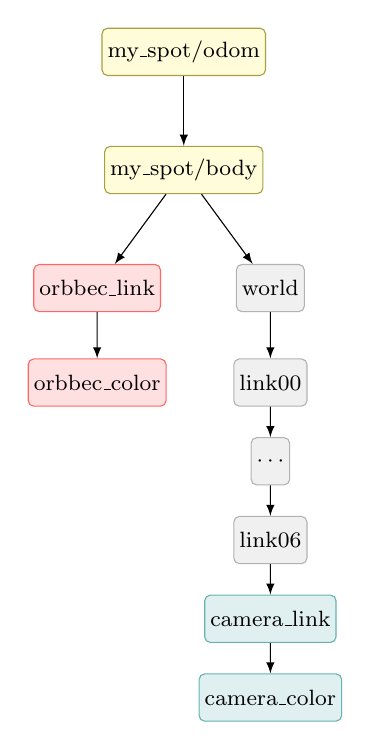
\begin{tikzpicture}[
    level 1/.style={sibling distance=40mm},
    level 2/.style={sibling distance=22mm},
    level 3/.style={level distance=12mm},
    level 4/.style={level distance=10mm},
    every node/.style={draw, rounded corners=2pt, font=\footnotesize,
                       inner sep=2pt, minimum height=6mm},
    edge from parent/.style={draw, -latex},
    spot/.style  = {fill=yellow!15,  draw=yellow!60!black},
    z1/.style    = {fill=gray!12,   draw=gray!60},
    orbbec/.style = {fill=red!12,   draw=red!60},
    rs/.style    = {fill=teal!12,   draw=teal!60},
  ]
  \node[spot] {my\_spot/odom}
    child { node[spot] {my\_spot/body}
      child { node[orbbec] {orbbec\_link}
        child { node[orbbec] {orbbec\_color} }
      }
      child { node[z1] {world}
        child { node[z1] {link00}
          child { node[z1] {$\cdots$}
            child { node[z1] {link06}
              child { node[rs] {camera\_link}
                child { node[rs] {camera\_color} }
              }
            }
          }
        }
      }
    };
\end{tikzpicture}

%  \caption{\ac{TF} frame tree. \texttt{my\_spot/odom} $\to$
%           \texttt{my\_spot/body} branches into the Orbbec chain and the Z1 arm
%           chain.}
%  \label{fig:frame_tree}
%\end{figure}

\subsection{Mission Management and System Integration}

The mission is orchestrated by a 13-state \ac{FSM}
(Fig.~\ref{fig:fsm}), organised into the four phases of
Section~\ref{sec:problem_formulation}. After Waiting TF and Idle ensure system
readiness, the \ac{FSM} enters Phase~A (Searching). The robot first walks the base
forward while adjusting body pitch to bring the patient into the cameras' field
of view---this is the SEARCHING state. When the RealSense detects a potential
torso, the system uses that coarse guidance to walk toward the detection and
adjust pitch, giving the Orbbec a clean observation window; we call this
SEMI\_LOCKING. If the Orbbec then confirms a lying patient with high
confidence, the system advances to LOCKING, where the NLF pipeline produces a
refined 3D skeleton and the coordinator collects approach point estimates.
Timeouts at any point revert to SEARCHING, ensuring the robot does not commit
to a false detection.

Phase~B (Approaching) begins once a stable lock is achieved. The robot first
drives toward the target while the anticipatory body scanner builds the torso
model---a state we call PRE\_APPROACH---then transitions to APPROACHING, where
the \ac{WBC} \ac{QP} coordinates base velocity and arm look-at control
concurrently, keeping the camera on the patient throughout the approach.

Phase~C (Exposure) starts after the approach handoff. An optional Waiting
Exposure gate lets the operator confirm before the scan begins. The system then
enters EXPOSURE\_SCANNING, executing a multi-view body surface inspection with
Grounding DINO injury detection at each grid point. Once the sweep is complete,
the \ac{FSM} moves to EXPOSURE\_REVIEW: the operator can click any grid point
in the web interface to trigger a full re-positioning and re-inspection,
remaining in this state until explicitly terminated.

Phase~D (\acs{FAST}) follows, with an analogous Waiting FAST gate for manual
confirmation. The SCANNING state executes ultrasound acquisition under
pre-planned body reconfiguration, one target at a time. When a target is
kinematically unreachable from the current posture, the system temporarily
enters WS\_EXTENSION, walking the base along the patient's body to extend the
workspace, then loops back to SCANNING with the new \ac{IK} solution.

Transitions are triggered by perception confidence (dashed edges in
Fig.~\ref{fig:fsm}) or geometric conditions (solid edges); the mission
completes by returning to Idle.

Fig.~\ref{fig:system_block} shows the complete system architecture in six
layers.  The Orbbec and RealSense \ac{RGBD} streams feed the Perception layer,
which runs YOLO-pose skeleton detection, Kalman-filtered 3D back-projection,
NLF 3D body pose estimation, surface estimation, and Grounding DINO injury
detection.  Perception outputs route to the 13-state Mission \ac{FSM}, which
enables four Planning modules: the Exposure Scanner, the \ac{FAST} Ultrasound
planner, the Body Pose Optimizer, and the Web UI for interactive review.  The
Control layer translates plans into actuation: the \ac{WBC} \ac{QP} publishes
base velocity $[v_x,\,\omega_z]$ to Spot and arm goals to the \ac{IK} Goal
Multiplexer; the Impedance Controller manages compliant contact during
\ac{FAST} scanning, publishing joint torques $\boldsymbol{\tau}$ directly to
the Z1.  The Z1 \ac{FSM} manages the arm's internal state
transitions---homing, look-at tracking, scanning trajectory execution, and
impedance-controlled contact---and synchronises with the \ac{WBC} coordinator.
Dashed arrows in the diagram denote operator-triggered or posture-optimisation
paths.  An emergency stop immediately halts the base and returns the arm to a
safe configuration.

\begin{figure*}[t]
  \centering
  \resizebox{\textwidth}{!}{% ============================================================
%  FSM DIAGRAM — 13 states, 4 columns
%  Requires: tikz
% ============================================================
\begin{tikzpicture}[
    node distance = 1.6cm and 1.8cm,
    auto,
    >=stealth,
    state/.style   = {rectangle, rounded corners=3pt, draw, minimum width=1.6cm,
                      minimum height=0.55cm, font=\tiny,
                      fill=white, thick, inner sep=2pt},
    search/.style  = {state, draw=orange!70, fill=orange!8},
    lock/.style    = {state, draw=red!60, fill=red!8},
    approach/.style = {state, draw=blue!70, fill=blue!8},
    expose/.style  = {state, draw=cyan!65, fill=cyan!8},
    review/.style  = {state, draw=teal!60, fill=teal!8},
    scan/.style    = {state, draw=green!60!black, fill=green!8},
    idle/.style    = {state, draw=gray!70, fill=gray!8},
    wait/.style    = {state, draw=violet!60, fill=violet!8, densely dashed},
    trans/.style   = {->, thick, font=\tiny},
    transd/.style  = {->, thick, dashed, font=\tiny},
    every label/.style = {font=\tiny}
  ]

  % ── Column 1: Init (x≈0.0) ──────────────────────────────────
  \node[idle]  (wtf)                                  {Waiting TF};
  \node[idle]  (idl)  [below=of wtf]                   {Idle};

  % ── Column 2: Search / Lock (x≈2.8) ─────────────────────────
  \node[search] (sr)  [right=2.8cm of idl]                    {Searching};
  \node[lock]   (sl)  [above=of sr]                            {Semi-locking};
  \node[lock]   (lk)  [right=of sl]                            {Locking};

  % ── Column 3: Approach + Exposure (x≈6.2) ──────────────────
  \node[approach] (pa) [right=2.2cm of lk]                     {Pre-approach};
  \node[approach] (ap) [below=of pa]                            {Approaching};
  \node[wait]     (we) [below=1.8cm of ap]                        {Wait. Exp.};
  \node[expose]   (es) [right=2.2cm of ap]                      {Exp. Scanning};
  \node[review]   (er) [below=of es]                            {Exp. Review};

  % ── Column 4: FAST (x≈10.2) ─────────────────────────────────
  \node[scan]    (sc) [right=2.2cm of es]                      {Scanning (FAST)};
  \node[wait]    (wf) [above=of sc]                            {Wait. FAST};
  \node[approach] (ws) [right=2.2cm of sc]                     {WS ext};

  % ── Transitions ─────────────────────────────────────────────

  % Init
  \draw[trans] (wtf) -- node[right]{\tiny TF ready} (idl);
  \draw[trans] (idl) -- node[above]{\tiny start} (sr);

  % Search / Lock
  \draw[trans] (sr)  -- node[left]{\tiny RS guided} (sl);
  \draw[trans] (sl)  -- node[above]{\tiny Orbbec} (lk);
  \draw[transd] (sl.west) -- ++(-0.5,0) |- node[pos=0.4,left]{\tiny timeout} (sr.west);
  \draw[trans] (sr)  -| node[above left,pos=0.7]{\tiny LYING} (lk);
  \draw[transd] (lk.south west) -- node[above left,pos=0.4,yshift=2pt]{\tiny timeout} (sr.north east);

  % Lock → Pre-approach
  \draw[trans] (lk)  -- node[above]{\tiny samples+ik} (pa);

  % Pre-approach → Approaching
  \draw[trans] (pa)  -- node[left]{\tiny EST/LOCKED} (ap);
  \draw[transd] (pa) to[loop right] node[right]{\tiny timeout} (pa);

  % Approaching → Exposure (conditional gate)
  \draw[trans] (ap.east) -- node[above,pos=0.3]{\tiny handoff} (es.west);
  \draw[transd] (ap) -- node[left]{\tiny man.\ gate} (we);

  % Waiting Exposure → Exposure Scanning
  \draw[trans] (we) -- node[above]{\tiny confirm} (es);

  % Exposure Scanning → Exposure Review
  \draw[trans] (es) -- node[right,near start]{\tiny /exp.\_ready} (er);

  % Exposure Review → FAST (conditional gate)
  \draw[trans] ([yshift=-0.2cm]er.east) -| node[above,pos=0.25]{\tiny terminate} ([xshift=-0.2cm]sc.south);
  \draw[transd] ([yshift=0.2cm]er.east) -- ++(0.8,0) |- node[left,pos=0.4]{\tiny man.\ gate} (wf.west);

  % Waiting FAST → Scanning
  \draw[trans] (wf.south) -- node[below right,pos=0.7]{\tiny confirm} (sc.north);

  % Scanning ↔ WS ext
  \draw[trans] (sc) -- node[above]{\tiny unreach.} (ws);
  \draw[trans] (ws) -- node[below]{\tiny ik\_done} (sc);

  % Complete → Idle (passes below all states)
  \draw[transd] ([xshift=+0.2cm]sc.south) -- ++(0,-2.5) -|
    node[pos=0.22,below]{\tiny complete} (idl.south);

  % ── Legend ──────────────────────────────────────────────────
  \node[state, draw=orange!70, fill=orange!8, minimum width=1.0cm,
        font=\tiny, inner sep=1pt] at (7.5, -5.7) {Search};
  \node[state, draw=red!60, fill=red!8, minimum width=1.0cm,
        font=\tiny, inner sep=1pt] at (9.0, -5.7) {Lock};
  \node[state, draw=blue!70, fill=blue!8, minimum width=1.0cm,
        font=\tiny, inner sep=1pt] at (10.5, -5.7) {Approach};
  \node[state, draw=cyan!65, fill=cyan!8, minimum width=0.9cm,
        font=\tiny, inner sep=1pt] at (12.0, -5.7) {Expose};
  \node[state, draw=teal!60, fill=teal!8, minimum width=0.9cm,
        font=\tiny, inner sep=1pt] at (13.5, -5.7) {Review};
  \node[state, draw=green!60!black, fill=green!8, minimum width=0.9cm,
        font=\tiny, inner sep=1pt] at (15.0, -5.7) {FAST};
  \draw[transd, thick] (16.0, -5.7) -- node[above,font=\tiny]{dashed} ++(1.0,0);

\end{tikzpicture}
}
  \caption{Mission \ac{FSM} with 13 states. Dashed transitions are
           perception-driven; solid transitions are geometry-driven.}
  \label{fig:fsm}
\end{figure*}

\begin{figure}[t]
  \centering
  \resizebox{\columnwidth}{!}{% ============================================================
%  SYSTEM BLOCK DIAGRAM — 5 columns + injury detection + web UI
% ============================================================
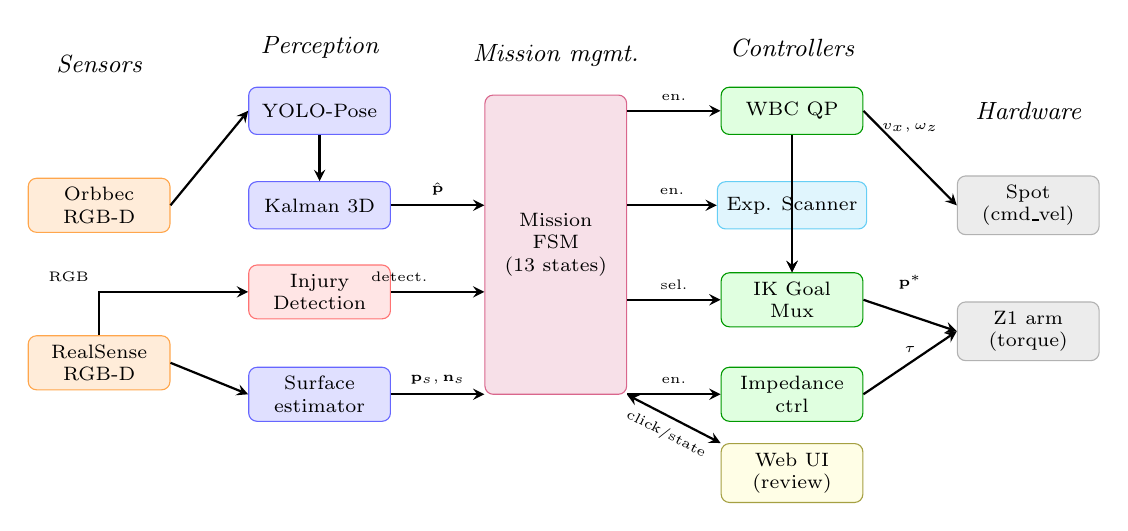
\begin{tikzpicture}[
    >=stealth,
    arr/.style    = {->, thick},
    arrb/.style   = {<->, thick},
    box/.style    = {rectangle, draw, rounded corners=3pt,
                     minimum width=1.8cm, minimum height=0.60cm,
                     font=\scriptsize, align=center, fill=white},
    sensor/.style = {box, fill=orange!15, draw=orange!70},
    percep/.style = {box, fill=blue!12,   draw=blue!60},
    injury/.style = {box, fill=red!10,    draw=red!55},
    fsmbox/.style = {box, fill=purple!12, draw=purple!60,
                     minimum width=1.8cm, minimum height=3.8cm},
    ctrl/.style   = {box, fill=green!12,  draw=green!60!black},
    expctrl/.style = {box, fill=cyan!12,  draw=cyan!60},
    web/.style    = {box, fill=yellow!10, draw=yellow!60!black},
    hw/.style     = {box, fill=gray!15,   draw=gray!60},
    lbl/.style    = {font=\small\itshape},
  ]

  % ── Column x: 0  2.8  5.8  8.8  11.8 ───────────────────────
  % ── Row y:  top rows between +2.6 and -2.4 ────────────────

  % SENSORS
  \node[sensor] (orb)  at ( 0.0,  1.0) {Orbbec\\RGB-D};
  \node[sensor] (rs)   at ( 0.0, -1.0) {RealSense\\RGB-D};

  % PERCEPTION
  \node[percep] (yolo) at ( 2.8,  2.2) {YOLO-Pose};
  \node[percep] (kf)   at ( 2.8,  1.0) {Kalman 3D};
  \node[injury] (inj)  at ( 2.8, -0.1) {Injury\\Detection};
  \node[percep] (surf) at ( 2.8, -1.4) {Surface\\estimator};

  % FSM
  \node[fsmbox] (fsm)  at ( 5.8,  0.5) {Mission\\FSM\\(13 states)};

  % CONTROLLERS
  \node[ctrl]  (wbc)  at ( 8.8,  2.2) {WBC QP};
  \node[expctrl] (exp) at (8.8,  1.0) {Exp. Scanner};
  \node[ctrl]  (mux)  at ( 8.8, -0.2) {IK Goal\\Mux};
  \node[ctrl]  (imp)  at ( 8.8, -1.4) {Impedance\\ctrl};

  % WEB UI
  \node[web] (webui) at ( 8.8, -2.4) {Web UI\\(review)};

  % HARDWARE
  \node[hw] (spot) at (11.8,  1.0) {Spot\\(cmd\_vel)};
  \node[hw] (z1)   at (11.8, -0.6) {Z1 arm\\(torque)};

  % ── Sensors → Perception ────────────────────────────────────
  \draw[arr] (orb.east)  -- (yolo.west);
  \draw[arr] (yolo.south) -- (kf.north);
  \draw[arr] (rs.east)   -- (surf.west);
  \draw[arr] (rs.north)  |- node[above left,font=\tiny]{RGB} (inj.west);

  % ── Perception → FSM ────────────────────────────────────────
  \draw[arr] (kf.east)   -- node[above,font=\tiny]{$\hat{\mathbf{p}}$}
             (fsm.west |- kf);
  \draw[arr] (inj.east)  -- node[above left,font=\tiny]{detect.}
             (fsm.west |- inj);
  \draw[arr] (surf.east) -- node[above,font=\tiny]{$\mathbf{p}_s,\mathbf{n}_s$}
             (fsm.west |- surf);

  % ── FSM → Controllers ───────────────────────────────────────
  \draw[arr] (fsm.east |- wbc) -- node[above,font=\tiny]{en.} (wbc.west);
  \draw[arr] (fsm.east |- exp) -- node[above,font=\tiny]{en.} (exp.west);
  \draw[arr] (fsm.east |- mux) -- node[above,font=\tiny]{sel.}(mux.west);
  \draw[arr] (fsm.east |- imp) -- node[above,font=\tiny]{en.} (imp.west);

  % ── WBC → Mux + Exp Scanner → Mux ──────────────────────────
  \draw[arr] (wbc.south) -- (mux.north);
  \draw[arr] (exp.south) -- (mux.north);

  % ── FSM ↔ Web UI ────────────────────────────────────────────
  \draw[arrb] (fsm.south east) -- node[below,font=\tiny,sloped]{click/state} (webui.north west);

  % ── WBC → Spot ──────────────────────────────────────────────
  \draw[arr] (wbc.east) --
           node[above,font=\tiny,yshift=2mm]{$v_x,\omega_z$} (spot.west);

  % ── Mux → Z1 ────────────────────────────────────────────────
  \draw[arr] (mux.east) --
             node[above,font=\tiny,yshift=2mm]{$\mathbf{p}^*$}
             (z1.west);

  % ── Imp → Z1 ────────────────────────────────────────────────
  \draw[arr] (imp.east) --
             node[above,font=\tiny]{$\boldsymbol{\tau}$}
             (z1.west);

  % ── Column labels ────────────────────────────────────────────
  \node[lbl] at ( 0.0,  2.8) {Sensors};
  \node[lbl] at ( 2.8,  3.0) {Perception};
  \node[lbl] at ( 5.8,  2.9) {Mission mgmt.};
  \node[lbl] at ( 8.8,  3.0) {Controllers};
  \node[lbl] at (11.8,  2.2) {Hardware};

\end{tikzpicture}
}
  \caption{System block diagram. The six-layer architecture spans sensors,
           perception, mission \ac{FSM}, planning, control, and hardware.
           Dashed arrows denote operator-triggered or posture-optimisation
           paths.}
  \label{fig:system_block}
\end{figure}

\subsection{Web-Based Operator Interface}

Full autonomy in emergency assessment is neither feasible nor desirable: the
operator must retain the ability to override or re-inspect regions of clinical
interest. \ac{TERESA} bridges this gap with a web interface that translates a
single 2D click on the Body Map into a 3D whole-body repositioning
command---posture optimisation, base navigation, and arm trajectory
replay---without manual teleoperation.

The \ac{TERESA} web interface provides dual-camera monitoring and robot control
via a browser-based dashboard. During exposure
review, the RealSense overlay renders the scan grid as clickable markers; each
click triggers a full re-positioning sequence---posture optimisation, settle,
and \ac{IK} trajectory replay---within the same \ac{ROS}~2 topic protocol used
for autonomous operation. A manual/automatic scan gate toggle allows the
operator to require explicit confirmation before advancing between mission
phases. All web commands are mirrored on the keyboard controller for
redundancy. Fig.~\ref{fig:web_interface} shows the interface during review.

\begin{figure}[t]
  \centering
  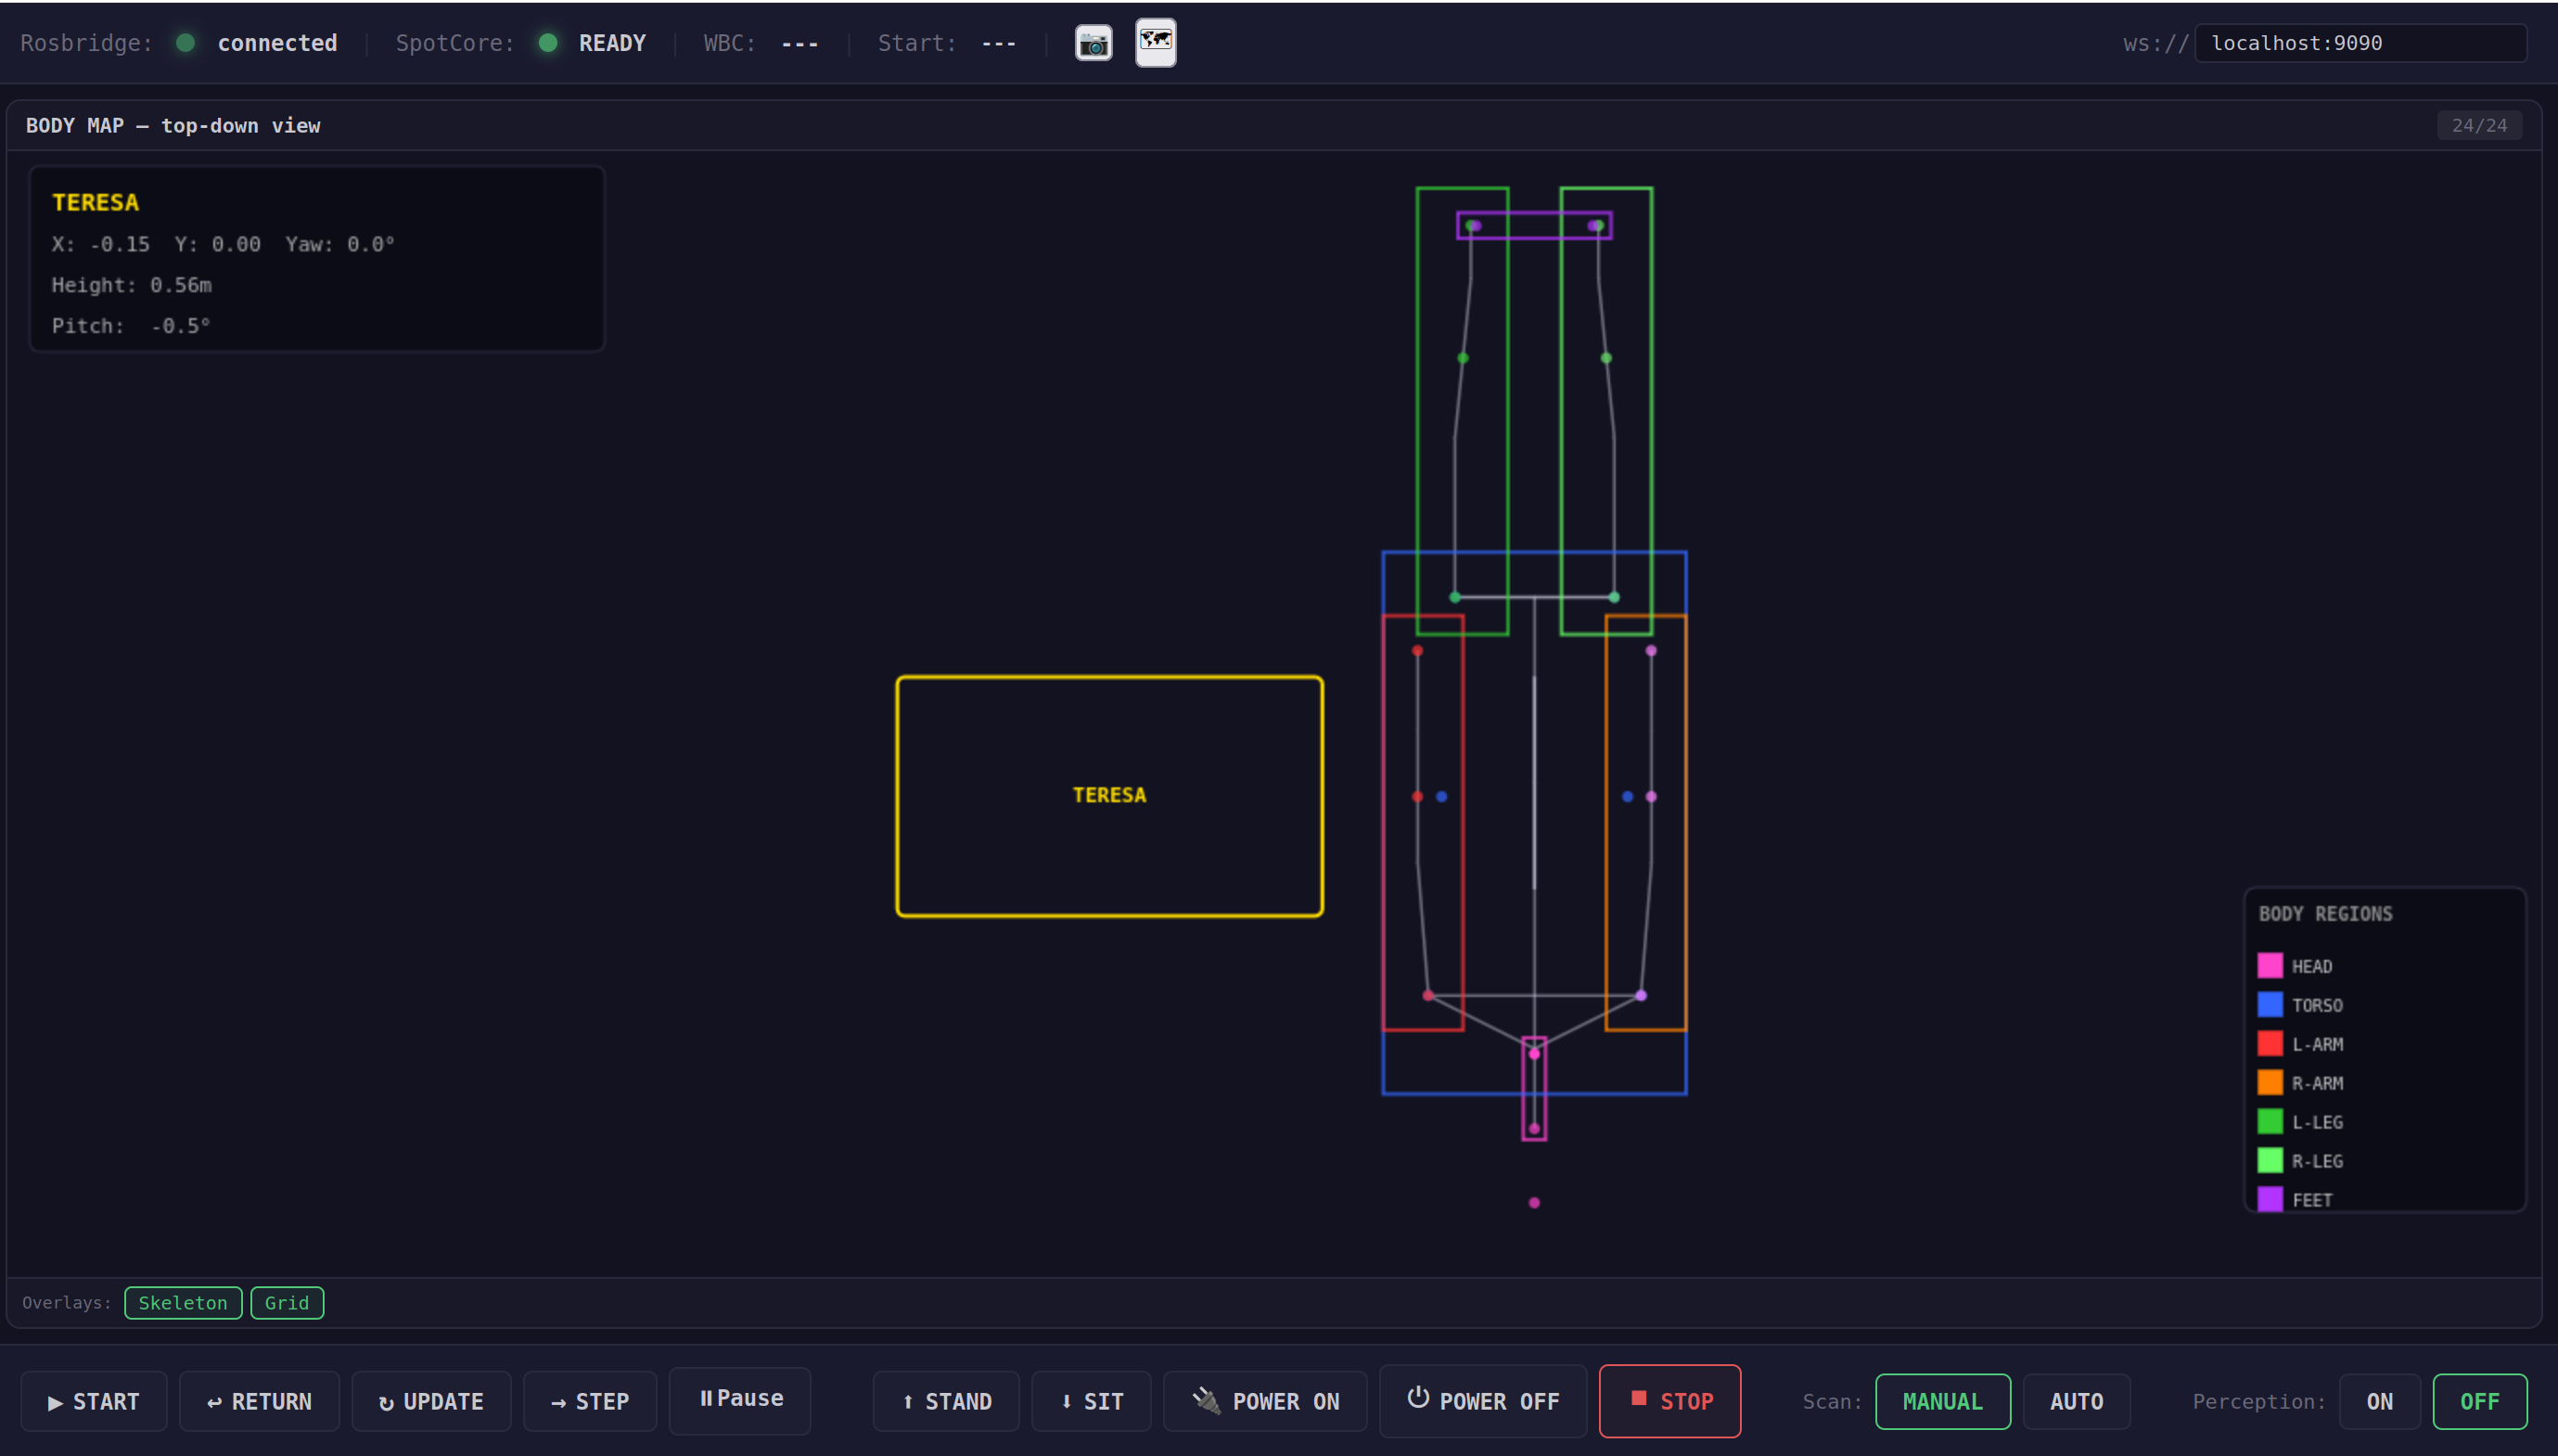
\includegraphics[width=\columnwidth]{figures/Web_interface}
  \caption{Web-based operator interface during the exposure scanning phase. The
           Body Map (top-down view) shows the patient mannequin skeleton with
           colour-coded body regions, the exposure scan grid points, and the Spot
           robot position (yellow). The info panel (top-left) displays Spot's
           current posture parameters. During exposure review, the operator can
           click any grid marker to command the robot to re-inspect that body
           region.}
  \label{fig:web_interface}
\end{figure}
